\documentclass[12pt, a4paper]{article}

\usepackage[left=3cm,top=3cm,right=2cm,bottom=2cm]{geometry}
\usepackage[brazilian]{babel}
\usepackage{amsfonts, amsmath, amssymb}
\usepackage{graphicx, float}

\title{(Universidade de São Paulo)\\
Trabalho 3:\\Equações Parabólicas e Hiperbólicas}

\author{Métodos Numéricos em Equações Diferenciais\\
Docente: Fabrício Simeoni de Sousa\\[.2cm]
\begin{tabular}{r@{\ }c@{\ }l}
    Kainã Alves Tureso      &-- &15466391\\
    Vinícius de Sá Ferreira &-- &15491650
\end{tabular}}

\date{\today}
\graphicspath{{../graphs}}

\renewcommand{\arraystretch}{1.3}
\newcommand{\bb}[1]{\mathbb{#1}}
\renewcommand{\bf}[1]{\mathbf{#1}}
\newcommand{\D}[1]{\Delta#1}
\renewcommand{\O}[1]{\mathcal{O} (#1)}
\newcommand{\Pe}{\bb{P}e}

\begin{document}

    \maketitle

    \section{EDP}
    Da EDP
    \begin{equation}
        u_t(x,t) + u_x(x,t) = \frac{1}{\bb{P}e} u_{xx}(x,t), \quad (x,t) \in [0,15] \times [0,12]
    \end{equation}
    definimos $x_j = j\D{x}$ e $t_n = n\D{t}$, com $j = 0,1,\ldots,N_x$ e $n = 0,1,\ldots,N_t$, então para $U_j^n \approx u(x_j,t_n)$ discretizamos

    \section{Discretizações}
    \subsection{Progressivas no tempo e centradas no espaço}
    \begin{equation}
        \begin{split}
            &\frac{u(x_j,t_{n+1})-u(x_j,t_n)}{\D{t}} + \O{\D{t}} + \frac{u(x_{j+1},t_n)-u(x_{j-1},t_n)}{2\D{x}} + \O{\D{x}^2}
            \\&= \frac{1}{\bb{P}e} \frac{u(x_{j+1},t_n)-2u(x_j,t_n)+u(x_{j-1},t_n)}{\D{x}^2} + \O{\D{x}^2}
        \end{split}
    \end{equation}

    que produz o método
    \begin{equation}
        \frac{U_j^{n+1}-U_j^n}{\D{t}} + \frac{U_{j+1}^n-U_{j-1}^n}{2\D{x}} = \frac{1}{\bb{P}e} \frac{U_{j-1}^n-2U_j^n+U_{j+1}^n}{\D{x}^2}
    \end{equation}

    ou, equivalentemente
    \begin{equation}
        \begin{split}
            U_j^{n+1} &= \left(\frac{\D{t}}{\bb{P}e\D{x^2}}+\frac{\D{t}}{2\D{x}}\right)U_{j-1}^n + \left(1-\frac{2\D{t}}{\bb{P}e\D{x^2}}\right)U_j^n + \left(\frac{\D{t}}{\bb{P}e\D{x^2}}-\frac{\D{t}}{2\D{x}}\right)U_{j+1}^n\\[.2cm]
            &= (\alpha+\beta)U_{j-1}^n + (1-2\alpha)U_j^n + (\alpha-\beta)U_{j+1}^n
        \end{split} \label{eq:centradas}
    \end{equation}
    onde $\alpha = \dfrac{\D{t}}{\bb{P}e\D{x^2}}$ e $\beta = \dfrac{\D{t}}{2\D{x}}$.

    \newpage
    
    Para as condições de contorno periódicas, definimos $U_{N_x+1}^n = U_0^n$, então:

    $j = 0$:
    \[U_0^{n+1} = (\alpha+\beta)U_{-1}^n + (1-2\alpha)U_0^n + (\alpha-\beta)U_{1}^n = (1-2\alpha)U_0^n + (\alpha-\beta)U_{1}^n + (\alpha+\beta)U_{N_x}^n\]

    $j = N_x$:
    \[U_{N_x}^{n+1} = (\alpha+\beta)U_{N_x-1}^n + (1-2\alpha)U_{N_x}^n + (\alpha-\beta)U_{N_x+1}^n = (\alpha-\beta)U_{0}^n + (\alpha+\beta)U_{N_x-1}^n + (1-2\alpha)U_{N_x}^n\]

    Portanto, para a forma matricial, teremos
    \begin{equation}
        \bf{U^{n+1}} = A\bf{U^n}
    \end{equation}
    onde $\bf{U^n} = \begin{bmatrix}
        U_0^n \\ U_1^n \\ U_2^n \\ \vdots \\ U_{N_x}^n
    \end{bmatrix}$ e $A = \begin{bmatrix}
        (1-2\alpha) & (\alpha-\beta) & 0 & \cdots & (\alpha+\beta)\\
        (\alpha+\beta) & (1-2\alpha) & (\alpha-\beta) & \cdots & 0\\
        0 & (\alpha+\beta) & (1-2\alpha) & \cdots & 0\\
        \vdots & \vdots & \ddots & \ddots & \ddots\\
        (\alpha-\beta) & 0 & \cdots & (\alpha+\beta) & (1-2\alpha)\\
    \end{bmatrix}$

    Da condição inicial $u(x,0) = \exp(-20{(x-2)}^2)+\exp(-{(x-5)}^2)$, obtemos na forma vetorial
    \[\bf{U_j^0} = \begin{bmatrix}
        \exp\{-20{(x_0-2)}^2\}+\exp\{-{(x_0-5)}^2\}\\
        \exp\{-20{(x_1-2)}^2\}+\exp\{-{(x_1-5)}^2\}\\
        \vdots\\
        \exp\{-20{(x_{N_x}-2)}^2\}+\exp\{-{(x_{N_x}-5)}^2\}\\
    \end{bmatrix}\]

    \subsubsection{Gráficos}
    Usando 430 pontos igualmente espaçados em $x$, obtemos $\Delta x = \dfrac{15}{430-1} \approx 3.4965 \cdot 10^{-2}$. Para satisfazer a desigualdade de estritamente menor, utilizamos $\varepsilon = 0.1$ de forma que 
    \begin{equation}
        \Delta t = (1-\varepsilon) \min\left\{ \dfrac{\Delta x^2}{\frac{2}{\bb{P}e} + \Delta x}, \Delta x \right\}, \label{eq:dt}
    \end{equation}
     logo:
    \begin{itemize}
        \item $\bb{P}e = 0.1 \Rightarrow \Delta t \approx 5.4919 \cdot 10^{-5}$
        \item $\bb{P}e = 1 \Rightarrow \Delta t \approx 5.4070 \cdot 10^{-4}$
        \item $\bb{P}e = 20 \Rightarrow \Delta t \approx 8.1525 \cdot 10^{-3}$
    \end{itemize}

    Assim, obtivemos os seguintes resultados:

    \begin{figure}[H]
        \centering
        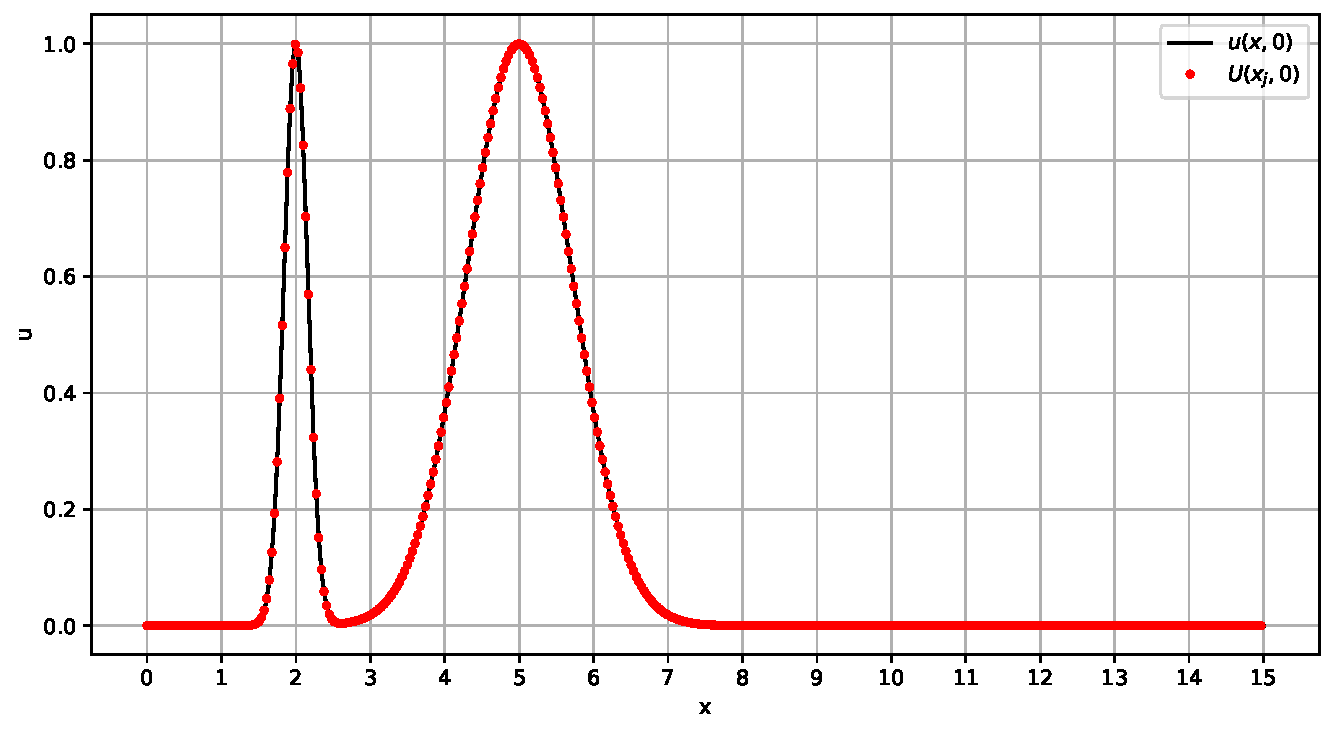
\includegraphics[width=0.85\textwidth]{initial_condition.pdf}
        \caption{Condição inicial}\label{fig:initial}
    \end{figure}
    
    \begin{figure}[H]
        \centering
        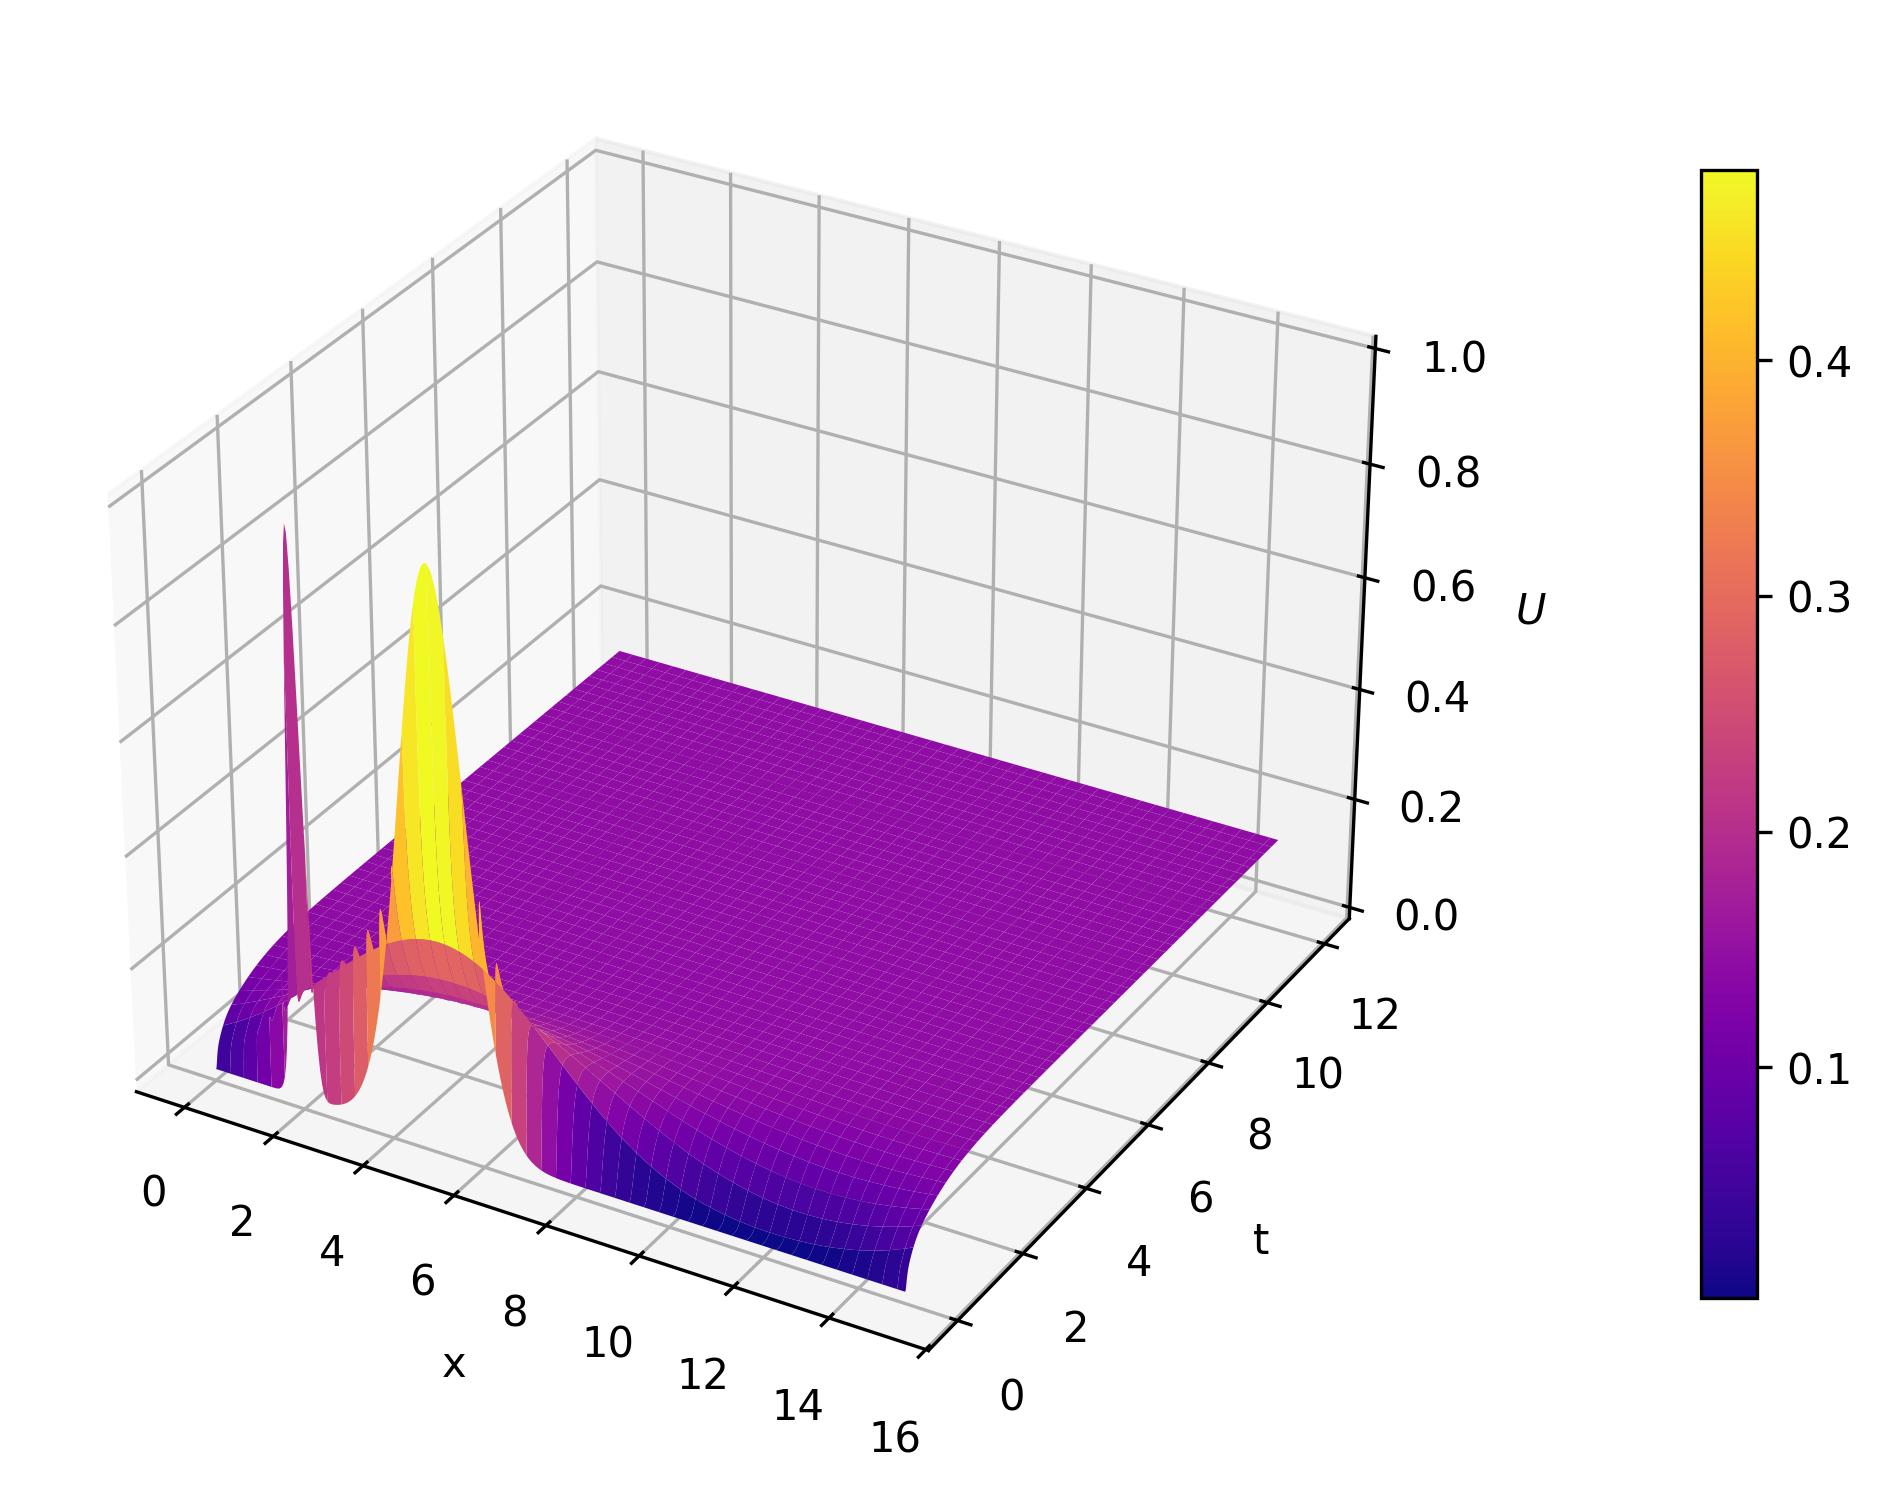
\includegraphics[width=0.85\textwidth]{surface_central_Pe=0.1.png}
        \caption{Solução numérica para $\bb{P}e = 0.1 \ll 1$ (Difusão dominante)}\label{fig:Pe0.1}
    \end{figure}

    \begin{figure}[H]
        \centering
        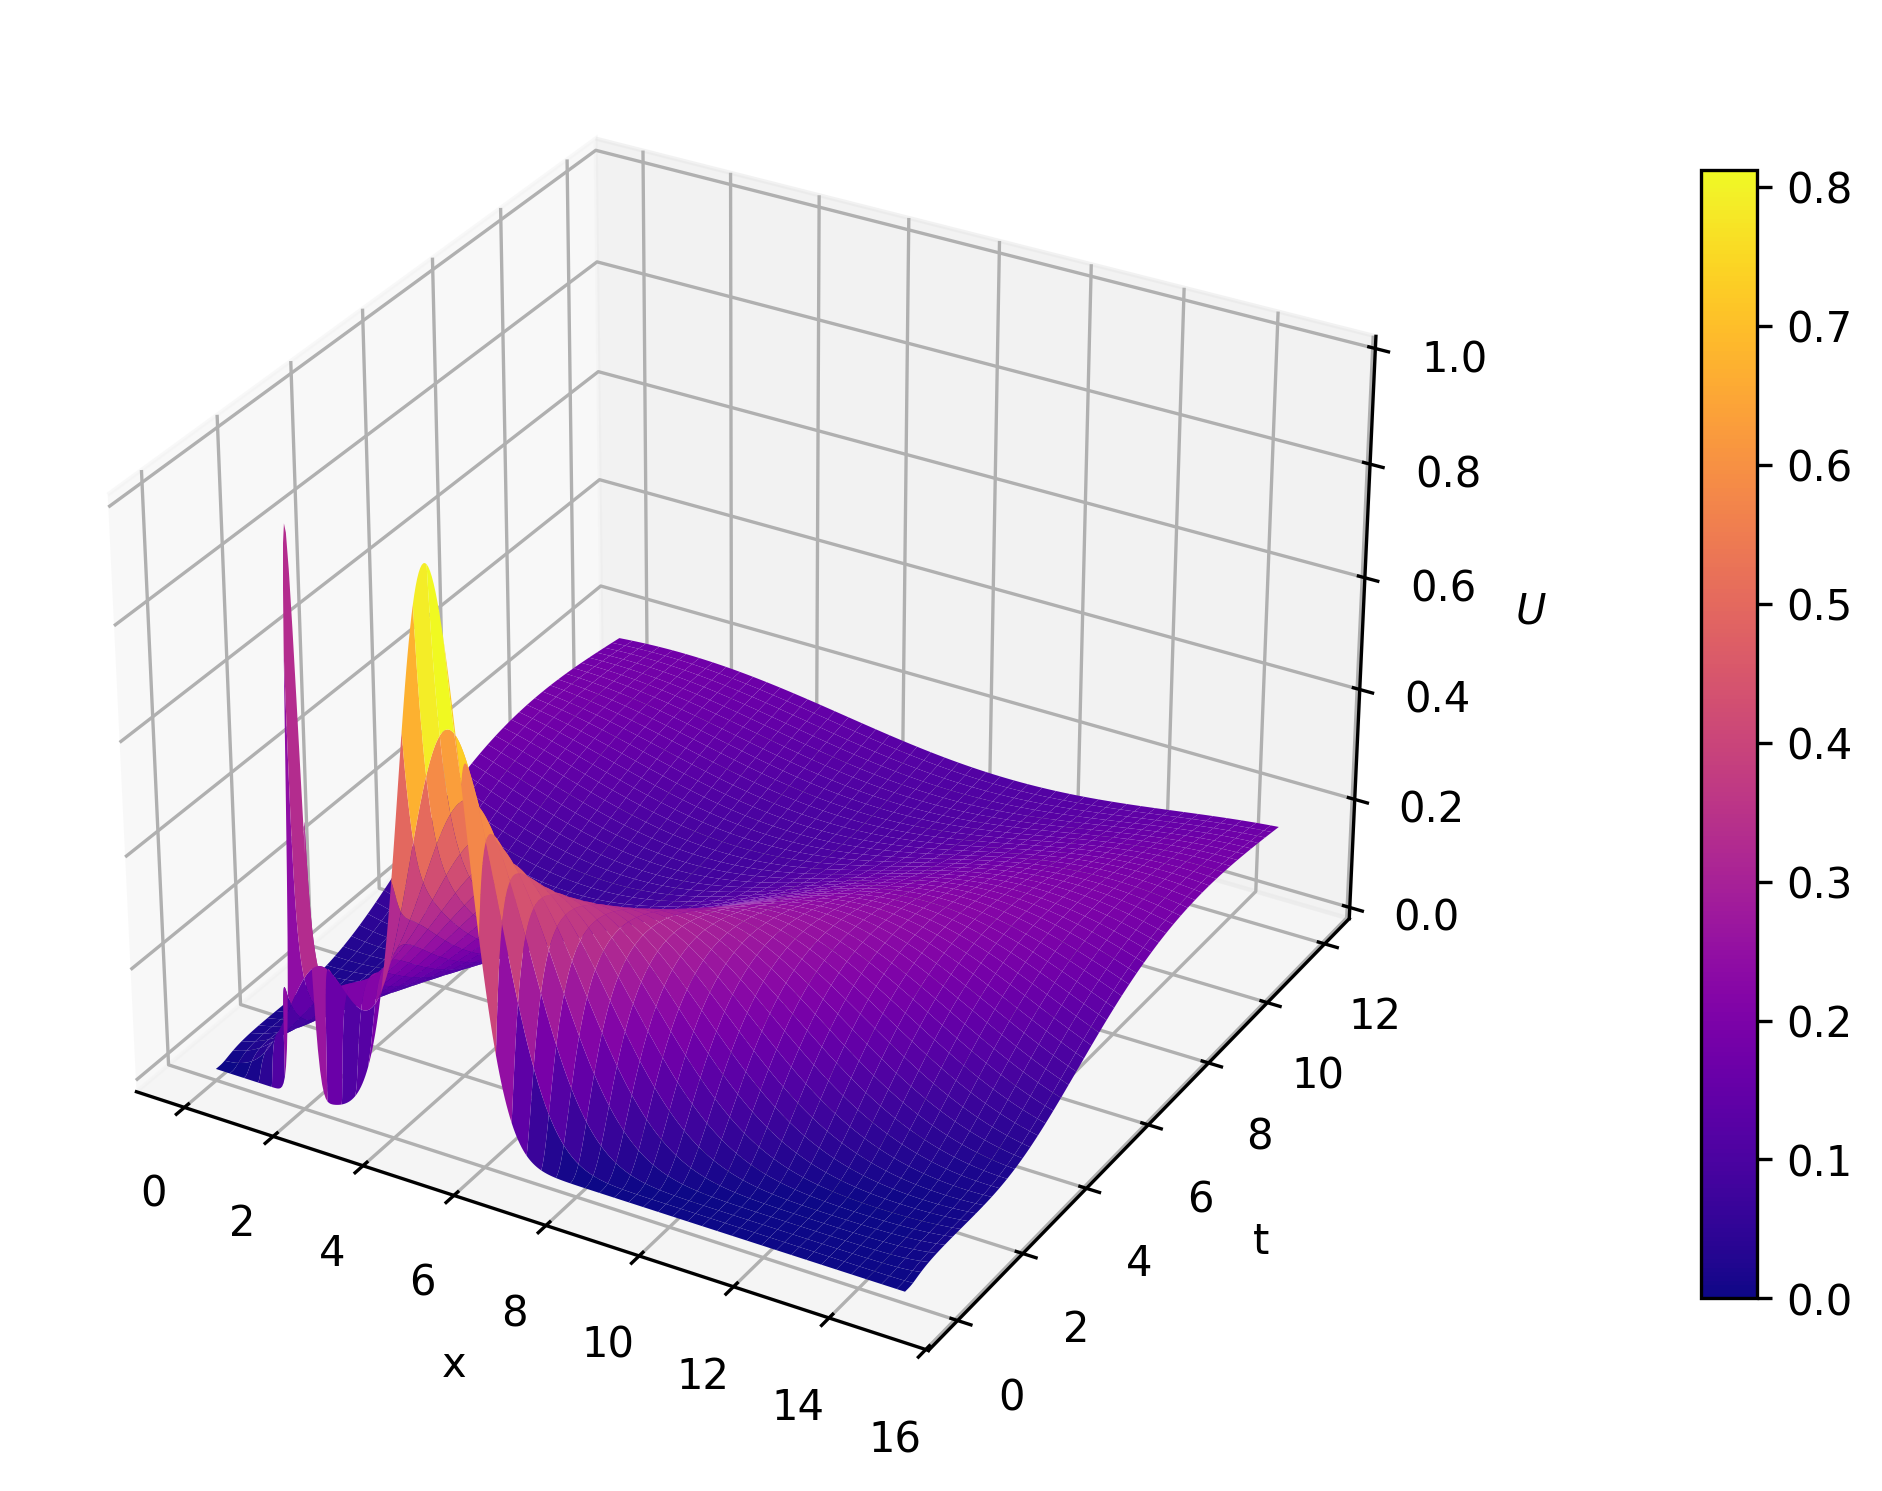
\includegraphics[width=0.85\textwidth]{surface_central_Pe=1.png}
        \caption{Solução numérica para $\bb{P}e = 1$ (Advecção-Difusão)}\label{fig:Pe1}
    \end{figure}

    \begin{figure}[H]
        \centering
        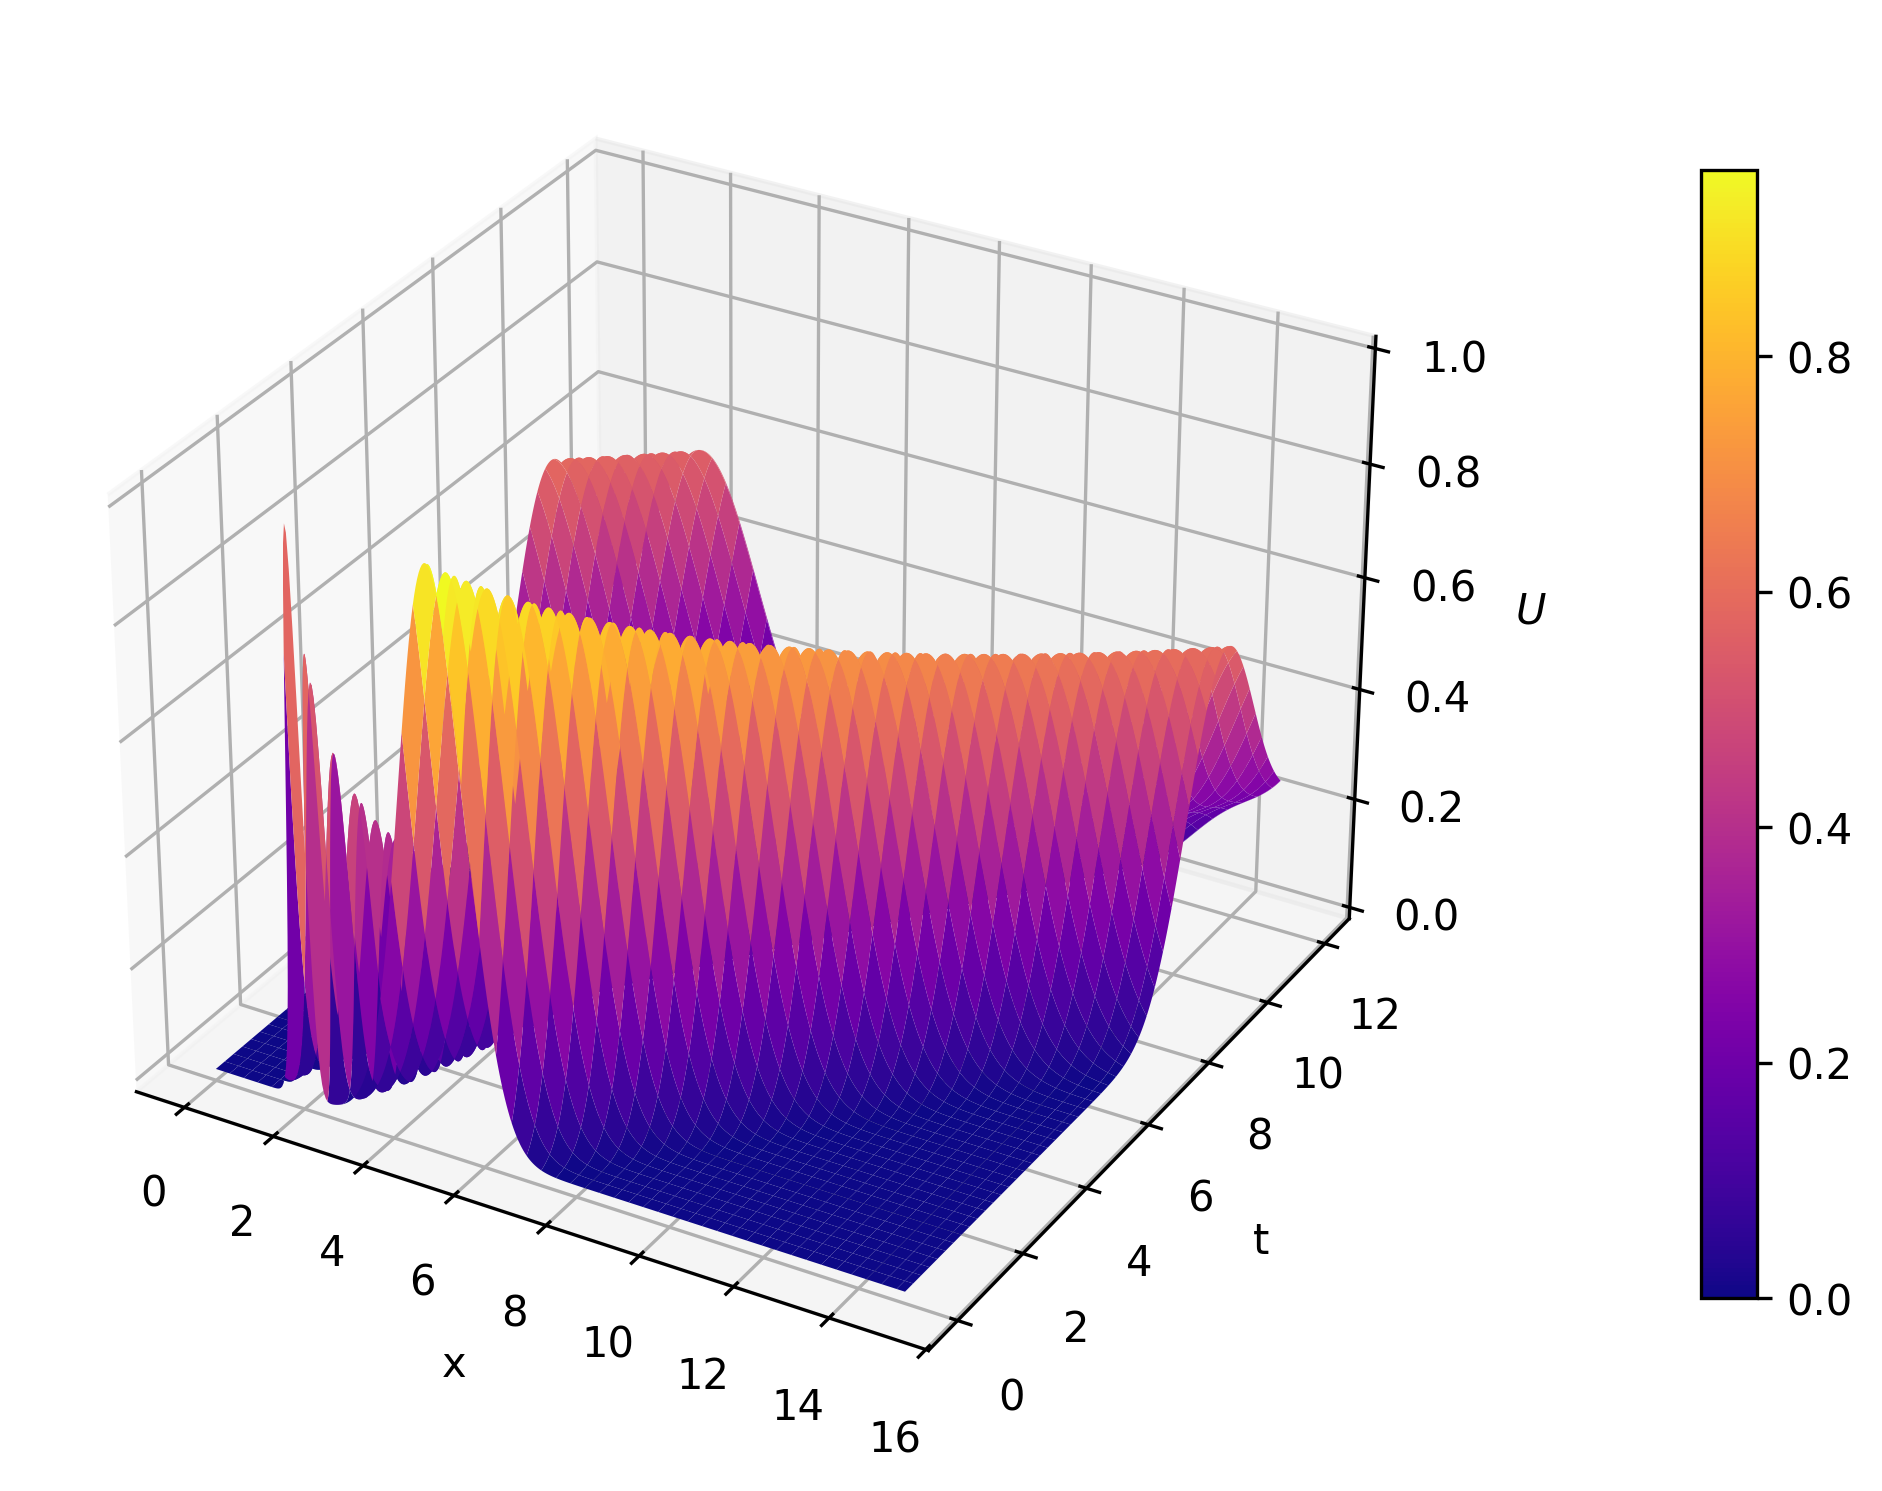
\includegraphics[width=0.85\textwidth]{surface_central_Pe=20.png}
        \caption{Solução numérica para $\bb{P}e = 20 \gg 1$ (Advecção dominante)}\label{fig:Pe20}
    \end{figure}

    \subsection{Upwind na derivada espacial}
    Como o termo que multiplica a primeira derivada espacial é positivo, pelo Upwind utilizamos diferenças regressivas para a derivada espacial, i.e.:
    \begin{equation}
        \begin{split}
            &\frac{u(x_j,t_{n+1})-u(x_j,t_n)}{\D{t}} + \O{\D{t}} + \frac{u(x_{j},t_n)-u(x_{j-1},t_n)}{\D{x}} + \O{\D{x}}
            \\&= \frac{1}{\bb{P}e} \frac{u(x_{j+1},t_n)-2u(x_j,t_n)+u(x_{j-1},t_n)}{\D{x}^2} + \O{\D{x}^2}
        \end{split}
    \end{equation}

    que produz o método
    \begin{equation}
        \frac{U_j^{n+1}-U_j^n}{\D{t}} + \frac{U_j^n-U_{j-1}^n}{\D{x}} = \frac{1}{\bb{P}e} \frac{U_{j-1}^n-2U_j^n+U_{j+1}^n}{\D{x}^2}
    \end{equation}

    ou, equivalentemente
    \begin{equation}
        \begin{split}
            U_j^{n+1} &= \left(\frac{\D{t}}{\bb{P}e\D{x}^2}+\frac{\D{t}}{\D{x}}\right)U_{j-1}^n + \left(1-\frac{2\D{t}}{\bb{P}e\D{x}^2}-\frac{\D{t}}{\D{x}}\right)U_j^n + \left(\frac{\D{t}}{\bb{P}e\D{x}^2}\right)U_{j+1}^n\\[.2cm]
            &= (\alpha+\gamma)U_{j-1}^n + (1-2\alpha-\gamma)U_j^n + \alpha U_{j+1}^n
        \end{split}
    \end{equation}
    onde $\alpha = \dfrac{\D{t}}{\bb{P}e\D{x^2}}$ e $\gamma = \dfrac{\D{t}}{\D{x}} = 2\beta$.

    \vspace{.3cm}

    Para as condições de contorno periódicas, definimos $U_{N_x+1}^n = U_0^n$, então:

    $j = 0$:
    \[U_0^{n+1} = (\alpha+\gamma)U_{-1}^n + (1-2\alpha-\gamma)U_0^n + \alpha U_{1}^n = (1-2\alpha-\gamma)U_0^n + \alpha U_{1}^n + (\alpha+\gamma)U_{N_x}^n\]

    $j = N_x$:
    \[U_{N_x}^{n+1} = (\alpha+\gamma)U_{N_x-1}^n + (1-2\alpha-\gamma)U_{N_x}^n + \alpha U_{N_x+1}^n = \alpha U_{0}^n + (\alpha+\gamma)U_{N_x-1}^n + (1-2\alpha-\gamma)U_{N_x}^n\]

    Portanto, para a forma matricial, teremos
    \begin{equation}
        \bf{U^{n+1}} = A\bf{U^n}
    \end{equation}
    onde $\bf{U^n} = \begin{bmatrix}
        U_0^n \\ U_1^n \\ U_2^n \\ \vdots \\ U_{N_x}^n
    \end{bmatrix}$ e $A = \begin{bmatrix}
        (1-2\alpha-\gamma) & \alpha & 0 & \cdots & (\alpha+\gamma)\\
        (\alpha+\gamma) & (1-2\alpha-\gamma) & \alpha & \cdots & 0\\
        0 & (\alpha+\gamma) & (1-2\alpha-\gamma) & \cdots & 0\\
        \vdots & \vdots & \ddots & \ddots & \ddots\\
        \alpha & 0 & \cdots & (\alpha+\gamma) & (1-2\alpha-\gamma)\\
    \end{bmatrix}$

    Da condição inicial $u(x,0) = \exp(-20{(x-2)}^2)+\exp(-{(x-5)}^2)$, obtemos na forma vetorial
    \[\bf{U_j^0} = \begin{bmatrix}
        \exp\{-20{(x_0-2)}^2\}+\exp\{-{(x_0-5)}^2\}\\
        \exp\{-20{_1(x-2)}^2\}+\exp\{-{(x_1-5)}^2\}\\
        \vdots\\
        \exp\{-20{(x_{N_x}-2)}^2\}+\exp\{-{(x_{N_x}-5)}^2\}\\
    \end{bmatrix}\]
    
    \newpage

    \subsubsection{Análise de Estabilidade}
    Pelo critério de Von Neumman, definimos $U_j^n = e^{i\omega_j}$ e $U_j^{n+1} = \zeta U_j^n = \zeta e^{i\omega_j}$. Logo, do método
    \[U_j^{n+1} = (\alpha+\gamma)U_{j-1}^n + (1-2\alpha-\gamma)U_j^n + \alpha U_{j+1}^n\]
    temos
    \[\zeta e^{i\omega_j} = (\alpha+\gamma) e^{i\omega_{j-1}} + (1-2\alpha-\gamma)e^{i\omega_j} + \alpha e^{i\omega_{j+1}}\]
    \[\begin{split}
        \zeta &= (\alpha+\gamma) e^{-i\omega} + (1-2\alpha-\gamma) + \alpha e^{i\omega}\\
        &= 1 + (e^{-i\omega}+e^{i\omega} - 2)\alpha + (e^{-i\omega} - 1)\gamma\\
        &= 1 + (2\cos(\omega) - 2)\alpha + (\cos(\omega)-i\sin(\omega) - 1)\gamma\\
        &= [1+(2\alpha+\gamma)(\cos(\omega)-1)] - i \gamma\sin(\omega)
    \end{split}\]
    e o método será estável se $|\zeta|^2 \leq 1$, logo:
    \[\begin{split}
        |\zeta|^2 &= {[1+(2\alpha+\gamma)(\cos(\omega)-1)]}^2 + {[\gamma\sin(\omega)]}^2\\
        &= 1 + 2(2\alpha+\gamma)(\cos(\omega)-1) + {(2\alpha+\gamma)}^2{(\cos(\omega)-1)}^2 + \gamma^2\sin^2(\omega)\\
    \end{split}\]
    \[= 1 - 4(2\alpha+\gamma)\sin^2(\omega/2) + {(2\alpha+\gamma)}^2{(-2\sin^2(\omega/2))}^2 + \gamma^2\sin^2(\omega)\]
    \[= 1 - (8\alpha+4\gamma)\sin^2(\omega/2) + (16\alpha^2+16\alpha\gamma+4\gamma^2)\sin^4(\omega/2) + \gamma^2\sin^2(\omega)\]
    \[= 1 - (8\alpha+4\gamma)\sin^2(\omega/2) + (16\alpha^2+16\alpha\gamma+4\gamma^2)\sin^4(\omega/2) + \gamma^2(4\sin^2(\omega/2)-4\sin^4(\omega/2))\]
    \[= 1 - (8\alpha+4\gamma-4\gamma^2)\sin^2(\omega/2) + (16\alpha^2+16\alpha\gamma+4\gamma^2-4\gamma^2)\sin^4(\omega/2)\]
    \[\leq 1 - (8\alpha+4\gamma-4\gamma^2) + (16\alpha^2+16\alpha\gamma)\]

    Portanto $|\zeta|^2 \leq 1 \iff - (8\alpha+4\gamma-4\gamma^2) + (16\alpha^2+16\alpha\gamma) \leq 0$, logo
    \[\begin{split}
        -8\alpha-4\gamma+4\gamma^2 + 16\alpha^2+16\alpha\gamma &\leq 0\\
        -2\alpha-\gamma+\gamma^2 + 4\alpha^2+4\alpha\gamma &\leq 0\\
        -(2\alpha+\gamma)+(4\alpha^2+4\alpha\gamma+\gamma^2) &\leq 0\\
        -(2\alpha+\gamma)+{(2\alpha+\gamma)}^2 &\leq 0\\
        (2\alpha+\gamma)(2\alpha+\gamma-1) &\leq 0\\
    \end{split}\]

    Como $\alpha,\gamma > 0$, então $2\alpha+\gamma > 0$. Portanto
    \[\begin{split}
        |\zeta|^2 \leq 1 \iff\quad 2\alpha+\gamma-1 &\leq 0\\
        2\dfrac{\D{t}}{\bb{P}e\D{x^2}} + \dfrac{\D{t}}{\D{x}} &\leq 1\\
        \D{t}\left(\dfrac{2}{\bb{P}e\D{x^2}} + \dfrac{1}{\D{x}}\right) &\leq 1\\
        \D{t}\left(\dfrac{2+\bb{P}e\D{x}}{\bb{P}e\D{x^2}}\right) &\leq 1\\
        \D{t}\left(\dfrac{\frac{2}{\bb{P}e}+\D{x}}{\D{x^2}}\right) &\leq 1\\
        \therefore \D{t} &\leq \dfrac{\D{x^2}}{\frac{2}{\bb{P}e}+\D{x}}\\
    \end{split}\]



    \section{Impacto do número de Péclet na discretização}
    Primeiro, notemos que a restrição $\Delta t < \min\left\{ \dfrac{\Delta x^2}{\frac{2}{\bb{P}e} + \Delta x}, \Delta x \right\}$ provém da análise de estabilidade e da Condição de CFL $\frac{|1|\D{t}}{\D{x}} < 1$. Sabendo que $\Pe > 0$, vemos que:
    \begin{align}
        \frac{\Delta x^2}{\frac{2}{\bb{P}e}+ \D{x}} < \frac{\Delta x^2}{\D{x}} = \D{x} \notag
    \end{align}

    Logo a restrição é simplesmente $\Delta t < \dfrac{\Delta x^2}{\frac{2}{\bb{P}e} + \Delta x}$

    Analisando $\alpha$ e $\beta$ na equação \ref{eq:centradas} e usando $\D{t}$ como em \ref{eq:dt}, temos:

    Para $\Pe \gg 1$:
    \begin{align}
        \D{t} = \frac{(1-\varepsilon)\D{x^2}}{\frac{2}{\Pe} + \D{x}} &\approx \frac{(1-\varepsilon)\D{x^2}}{\D{x}} = (1-\varepsilon) \D{x} \notag \\
        \alpha = \frac{\D{t}}{\Pe \D{x^2}} &\approx \frac{(1-\varepsilon) \D{x}}{\Pe \D{x^2}} = \frac{(1-\varepsilon)}{\Pe \D{x}} \le \frac{1}{\Pe \D{x}} \ll \frac{1}{\D{x}} \notag \\
        \beta = \frac{\D{t}}{2 \D{x}} &\approx \frac{(1- \varepsilon) \D{x}}{2 \D{x}} = \frac{(1 - \varepsilon)}{2} \notag
    \end{align}

    Para $\Pe \ll 1$:
    \begin{align}
        \D{t} = \frac{\Pe (1-\varepsilon)\D{x^2}}{2 + \Pe \D{x}} &\approx \frac{\Pe (1-\varepsilon)\D{x^2}}{2} \notag \\
        \alpha = \frac{\D{t}}{\Pe \D{x^2}} &\approx \frac{\Pe (1-\varepsilon)\D{x^2}}{2\Pe \D{x^2}} = \frac{1-\varepsilon}{2} \notag \\
        \beta = \frac{\D{t}}{2 \D{x}} &\approx \frac{\Pe (1-\varepsilon)\D{x^2}}{4\D{x}} = \frac{\Pe(1-\varepsilon)\D{x}}{4} \ll \frac{\D{x}}{4} \notag
    \end{align}

    \subsection{Discretização centrada}
    Quando $\Pe \gg 1$, utilizando as aproximação acima, temos $\alpha \approx 0$ e podemos reescrever a equação \ref{eq:centradas} como:
    \[
        U_j^{n+1} \approx \beta U_{j-1}^n + U_j^n -\beta U_{j+1}^n = U_j^n + \frac{\D{t}}{2\D{x}}(U_{j-1}^n - U_{j+1}^n)
    \]

    que é um método consistente com a equação $u_t(x,t) + u_x(x,t) = 0$, ou seja, a EDP original sem o termo difusivo, como esperado. Apesar disso, esse método é incondicionalmente instável, podendo ser facilmente visto com uma análise de Von Neumann. Ou seja, podemos dizer que, quando $\Pe \to \infty$, o método é instável. Isso poderá ser visto melhor na seção \ref{sec:inst}.

    Quando $\Pe \ll 1$, $\beta \approx 0$, logo, obtemos:
    \[
        U_j^{n+1} \approx \alpha U_{j-1}^n + (1 - 2\alpha) U_{j}^n + \alpha U_{j+1}^n = U_{j}^n + \frac{1}{\Pe}\frac{\D{t}}{\D{x^2}}(U_{j-1}^n - 2 U_{j}^n + U_{j-1}^n)
    \]
    Que é consistente com a equação $u_t(x,t) = \frac{1}{\Pe} u_{xx}(x,t)$ e condicionalmente estável.

    \subsection{Upwind na derivada espacial}
    Lembrando que $\gamma = 2\beta$, para $\Pe \gg 1$:
    \[
        U_j^n \approx \gamma U_{j-1}^n + (1 - \gamma)U_j^n = U_j^n -\frac{\D{t}}{\D{x}} (U_j^n - U_{j-1}^n)
    \]

    Que é consitente com a equação original sem o termo difusivo e estável quando a condição CFL é satisfeita.

    Para $\Pe \ll 1$:
    \[
        U_j^n \approx \alpha U_{j-1}^n + (1-2\alpha)U_j^n + \alpha U_{j+1}^n
    \]

    Obtemos o mesmo resultado que o caso $\Pe \ll 1$ para a discretização centrada.


    \subsection{Instabilidade para número de Péclet grande}
    \label{sec:inst}

\end{document}